\section{Methodology}
\figref{system_architecture} shows the architecture of the proposed system which takes as input multi-view color images of an object with known poses and outputs a triangle mesh of the object $ T = (V, F) $ where $ V = \{ v_i \in \mathbb{R}^3\} $ is the set of vertex coordinates and $ F \subseteq V \times V \times V $ is the set of faces.
The multi-view voxel grid prediction module (\subsecref{multiview_voxel}) first predicts a coarse voxel grid of the object.
The voxel grid is converted to mesh representation by cubify operation which is further refined by the mesh refinement module (\subsecref{mesh_refinement}).
A series of Graph Convolution Networks (GCN) deforms the cubified voxel grid to obtain surface mesh.
The GCNs use multi-view contrastive depth features from concatenated predicted and rendered depth along with RGB features as input to deform the input mesh.
Depth images are predicted using an extended MVSNet network~\cite{yao2018mvsnet}.
The multi-view features are fused using attention mechanism.

\subsection{Multi-view Voxel Grid Prediction}
\label{subsec:multiview_voxel}

\paragraph{Single-view Voxel Grid Prediction}
For each of the input single RGB image, we first generate the voxel occupancy grid of the target object.
Specifically, the single-view voxel branch adopts the approach proposed in~\cite{gkioxari2019meshrcnn} which consists of a ResNet feature extractor and a fully convolutional voxel grid prediction network. 
Here, we set the resolution of the generated voxel occupancy grid as 48 $\times$ 48 $\times$ 48. 
The voxel prediction networks for all viewpoints share the same weights.
% following Mesh R-CNN~\cite{gkioxari2019meshrcnn}.

\paragraph{Probabilistic Occupancy Grid Merging}\vspace{-4mm}
Voxel occupancy grid predicted from a single viewpoint suffers from occlusion and limited visibility.
In order to fuse voxel grids from different viewpoints we take inspiration from occupancy map building techniques in robotics~\cite{grisetti2007improved,konolige1997improved} and propose a probabilistic occupancy grid merging method which merges the voxel grids from each input viewpoint probabilistically to obtain the final voxel grid output.
This allows occluded regions in one view to be estimated from other views where those regions are visible as well as increase the confidence of prediction in overlapping regions.
Occupancy probability of each voxel is represented by $p(x)$ which is converted to log-odds (logit):
% \footnote{In practice the \emph{voxel branch} directly predicts the log-odds instead of probabilities}

\begin{equation}
    l(x) = log \frac{p(x)}{1 - p(x)}
    \label{equ:logodds}
\end{equation}

Bayesian update on the probabilities reduce to simple summation of log likelihoods~\cite{konolige1997improved}. Hence, the multi-view log-odds of a voxel is given by:

\begin{equation}
    l(x) = l_1(x) + l_2(x) + ... + l_n(x)
    \label{equ:logodds_sum}
\end{equation}

\noindent where $l_i$ is the voxel's log-odds in view $i$ and $n$ is the number of input views.
The final voxel probability $x$ is obtained by applying the inverse function of \equref{logodds} which is a sigmoid function.
% The final probability of the voxel $x$ can be obtained by applying the inverse function of \equref{logodds} which is a sigmoid function.
\siyu{Provide some intermediate visual results of merged occupancy grid and cubified meshes.}

\subsection{Mesh Refinement}
\label{subsec:mesh_refinement}
The cubified mesh from the voxel branch only provides a coarse reconstruction of the object's surface. 
We then apply the graph convolutional network in which the mesh vertex and edges are represented by the graph nodes and edges respectively, to deform the mesh to more accurate positions based on the RGB and contrastive depth features.\siyu{In the experimental section, provide some intermediate results of meshes after different iterations of GCN refinement.}

\label{subsec:depth_prediction}
\paragraph{Multi-View Depth Estimation}\vspace{-4mm}
To obtain the depth image of each RGB image, we iteratively regard each view as the reference and apply the standard MVSNet~\cite{yao2018mvsnet}.
In implementation, we discard the policy of view selection, and set the number of depth hypothesis to $48$ which is equivalent to a resolution of $25$ mm.

% We extend MVSNet~\cite{yao2018mvsnet} and predict the depth maps of all views since the original implementation predicts depth of only one reference view.
% This is achieved by transforming the feature volumes to each view's coordinate frame using homography warping
% and applying identical cost volume regularization and depth regression on each view.
% Detailed network architecture diagram of this module is provided in the appendix.


% which constructs a regularized 3D cost volumes
% to estimate the depth map of the reference view.
% Here, we extend MVSNet to predict the depth maps of all views instead of only the reference view.

% This allows the reuse of pre-regularization feature volumes for efficient multi-view depth prediction invariant to the order of input images.

\paragraph{GCN-based Mesh Deformation}\vspace{-4mm}
Following the prestigious previous works~\cite{wang2018pixel2mesh,wen2019pixel2mesh++}, a graph convolution deforms mesh vertices by propagating features from neighboring vertices by applying:
\begin{equation}
f_{i}^{'} = ReLU(W_0f_i + \sum_{j \in \mathcal{N}(i)} W_1 f_j),
\end{equation}
where $\mathcal{N}(i)$ is the set of neighboring vertices of the \emph{i}-th vertex in the mesh, $f_{\{\}}$ represents the feature vector of a vertex, and $W_0$ and $W_1$ are learnable parameters of the model.
The features pooled from multi-view images (discussed in subsequent paragraphs) along with 3D coordinates of the vertices in world frame are used as features of the graph nodes.
Series of Graph-based Convolutional Network (GCN) blocks are applied to deform a mesh at the current stage to the next stage, starting with the cubified voxel grids.
Each GCN block utilizes several graph convolutions to transform the vertex features along with a final vertex refinement operation where the features along with vertex coordinates are further transformed as:
\begin{equation}
v_i^{'} = v_i + tanh(W_{vert}[f_i;v_i]).
\end{equation}
Here, $v_i$ and $v_i^{'}$ represent the vertex coordinates before and after each refinement operation, and the matrix $W_{vert}$ is another learnable parameter to obtain the deformed mesh.

\label{subsec:contrastive_depth_feature_extraction}
\paragraph{Contrastive Depth Feature Extraction}\vspace{-4mm}
\begin{figure}[th!]
    \begin{center}
        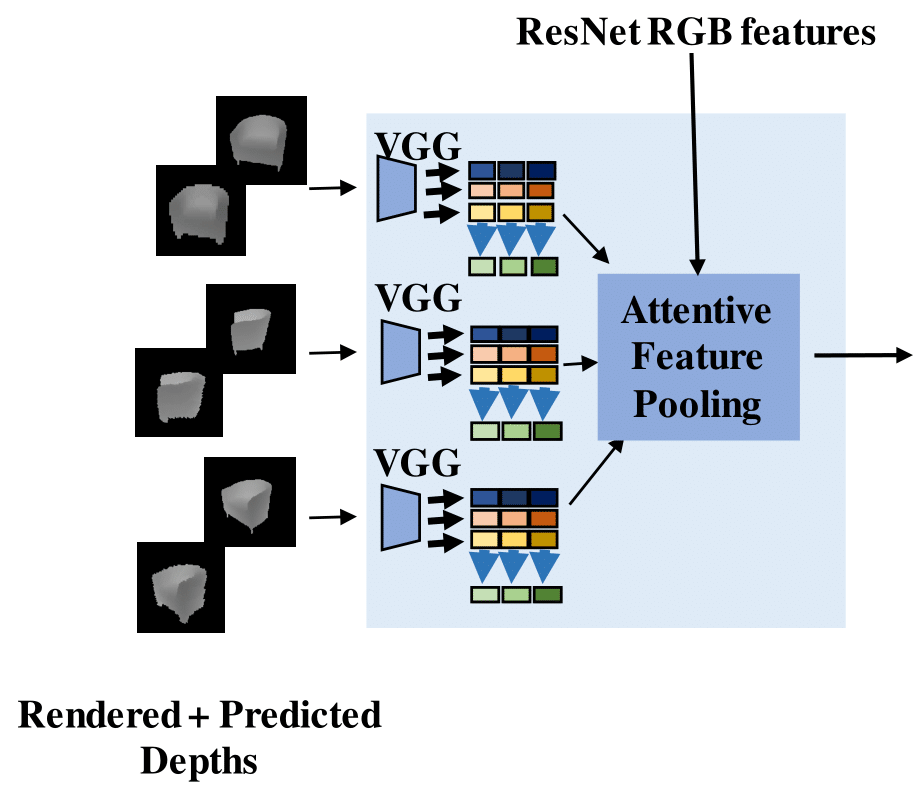
\includegraphics[width=0.8\linewidth]{imgs/contrastive_feature_extractor.png}
    \end{center}
        \caption{Contrastive feature extraction. Rendered depths of the current shape along with the predicted depths for each view are concatenated and VGG-based feature extractor is applied. Then along with the ResNet RGB features, the multi-view features are pooled using attentive feature pooling and used by GCN for deforming the shape}
        \label{fig:contrastive_feature_extractor}
\end{figure}

Inspired by the work~\cite{yao2020front2back} that incorporating intermediate and image-centric 2.5D representations instead of directly generating 3D shapes from only RGB images~\cite{wang2018pixel2mesh,wen2019pixel2mesh++} can improve 3D reconstruction quality.
As shown in Figure~\ref{fig:contrastive_feature_extractor}, we therefore propose to formulate the features of graph nodes using depth images as the additional inputs alongside with the RGB features.
At a single viewpoint, we consider two sources of depth images, namely the rendered depth from the meshes at different GCN stages and the corresponding input depth from multi-view stereo.
We apply the approach proposed in~\cite{kato2018renderer} for differentiable rendering.
Afterwards, we propose a contrastive feature extractor which contrasts the rendered depth of the current mesh against the input depth from multi-view stereo and guides the GCN to reason about the deformation.
We use VGG-16~\cite{simonyan2014vgg} as our contrastive depth feature extraction network.
Given the 2D feature maps, the feature vector of each graph node can be obtained by projecting its 3D coordinate to the corresponding feature map using known camera parameters.

% Specifically, we render the meshes at different GCN stages to depth image at all the input views using~\cite{kato2018renderer} and use them along with predicted depths for depth feature extraction. We call this form of depth input \texttt{contrastive depth} as it contrasts the rendered depths of the current mesh against the predicted depths and allows the network to reason about the deformation better than when using predicted depth or color images alone.
% construct the feature vector from semantic features of the input color images~\cite{wang2018pixel2mesh}, we formulate the input for feature extraction network using geometry representations.
% However, works similar to Pixel2Mesh~\cite{wang2018pixel2mesh} construct the feature vector from semantic features of the input color images. Here, we formulate the input for feature extraction network using geometry representations. Specifically, we render the meshes at different GCN stages to depth image at all the input views using~\cite{kato2018renderer} and augment them as additional inputs for depth feature extraction.
% We call this form of depth input \emph{contrastive depth} as it contrasts the rendered depths of the current mesh against the predicted depths and constrain the deformed mesh in a coarse-to-fine manner.
% Along with the contrastive depth features, we also use the RGB features from ResNet calculated for voxel branch as input for mesh deformation as well.

% and allows the network to reason about the deformation required better than when using predicted depths alone.
% Multiple methods for augmenting the two depths were tried among which using concatenated rendered and predicted depth as input for depth feature extraction gave the best result.
% Along with the contrastive depth features, we also use the RGB features from ResNet calculated for voxel branch as input for mesh deformation as well.

\paragraph{Attention-based Multi-View Feature Pooling}\vspace{-4mm}
In order to fuse multi-view contrastive depth features, we formulate an attention module by adapting multi-head attention mechanism originally designed for sequence to sequence machine translation using transformer architecture~\cite{vaswani2017attention}.
We choose multi-head attention as our feature pooling method since it allows the model to attend information from different representation subspaces of the features by training multiple attentions in parallel.
This method is also invariant to the order and number of input views.

% \rakesh{Transformer architecture was proposed in multi-head attention paper, it doesn't need a separate citation}
% In a transformer architecture the encoder hidden state is mapped to lower dimension key-value pairs (\textbf{K}, \textbf{V})
% while the decoder hidden state is mapped to a query vector \textbf{Q} using independent fully connected layers.
% The encoder hidden state in our case is the multi-view features while the decoder hidden state is the mean of the multi-view features.
% The attention weights are computed using scaled-dot product:
% \begin{equation}
%     Attention(\mathbf{Q}, \mathbf{K}, \mathbf{V}) = softmax(\frac{\mathbf{Q} \mathbf{K}^{T}}{\sqrt{N}}) \mathbf{V}
%     \label{equ:attention}
% \end{equation}
% \noindent where $N$ is the number of input views.

% Multiple attention heads are used which are concatenated and transformed to obtain the final output
% \begin{align}
%     head_i = Attention(\mathbf{Q} \mathbf{W}^{Q}_{i}, \mathbf{K} \mathbf{W}^{K}_{i}, \mathbf{V} \mathbf{W}^{V}_{i}) \label{equ:attention_head} \\
%     MultiHead(\mathbf{Q}, \mathbf{K}, \mathbf{V}) = [head_1; ...; head_h] \mathbf{W}^0 \label{equ:multihead_attention}
% \end{align}

% \noindent where multiple $\mathbf{W}$ are parameters to be learned,
% $h$ is the number of attention heads and $i\in[1,h]$.

% We refer our readers to~\cite{vaswani2017attention} for further technical details.


% instead of other forms of attention (e.g.~\cite{chorowski2015attention,luong2015effective}) because


% The network architectures of the GCN blocks are identical to Mesh R-CNN's implementation.
% We refer readers to~\cite{wang2018pixel2mesh,gkioxari2019meshrcnn} for further details.

% \rakesh{Differentiable Depth Rendering is just "Neural Renderer" without any change. This has already been covered in system overview}
% \subsection{Differentiable Depth Rendering}
% In order to add constrains of all intermediate predicted meshes, previous mesh generation methods~\cite{wang2018pixel2mesh} add loss terms to prevent the meshes deform too much. Here, we refer Neural Renderer~\cite{kato2018renderer} to differentiably render predicted meshes to depth images at all the input views.
% It approximates the gradients for rendering a mesh enabling back-propagation of losses defined on the rendered depths.
% % More recently methods that render depth without approximating the gradients have been proposed~\cite{liu2019soft};
% % but since it does not support depth rendering we use Neural Renderer.
% Note that any differentiable depth renderer can be used in its place.
%
% Prior works~\cite{kato2018renderer,liu2019soft} have used differentiable renderers in order to reconstruct 3D objects.
% These work rely solely on the rendered images or silhouettes for reconstruction.
% Since we directly supervise on 3D models during training, we use the rendered depths only for regularization.
% Specifically, the difference between the rendered depths and predicted depths at corresponding viewpoints are used as loss terms.
% The exact loss functions are described in \subsecref{losses}.

\subsection{Loss functions}
\label{subsec:losses}
% For training the mesh generation, we use the loss terms from~\cite{wang2018pixel2mesh} along with new losses based on our formulation.

\paragraph{Mesh losses}
To constrain the mesh predicted by each GCN block $P$ to resemble the ground truth $Q$, we use three mesh loss functions the same as~\cite{wang2018pixel2mesh}.
The first loss measures the Chamfer distance~\cite{fan2017point} between the nearest neighbor mesh vertices $\Lambda$, and deforms vertices to correct positions. 
It is defined as:

\begin{footnotesize}
\begin{equation}
\mathcal{L}_{\text{chamfer}}(P, Q) = |P|^{-1} \!\!\!\!\!\!\!\!\sum_{(p, q) \in \Lambda_{P,Q}}\!\!\!\!\!\!\!\!{||p-q||^{2}} + |Q|^{-1} \!\!\!\!\!\!\!\!\sum_{(q, p) \in \Lambda_{Q,P}}\!\!\!\!\!\!\!\!{||q-p||^{2}},
\end{equation}
\end{footnotesize}

\noindent Furthermore, to encode the local higher order surface properties, the normal loss function is defined as:

\begin{footnotesize}
\begin{equation}
\mathcal{L}_{\text{normal}}(P, Q) = -|P|^{-1}\!\!\!\!\!\!\!\! \sum_{(p, q) \in \Lambda_{P,Q}}\!\!\!\!\!\!\!\!{|u_p \cdot u_q|} - |Q|^{-1}\!\!\!\!\!\!\!\! \sum_{(q, p) \in \Lambda_{Q,P}}\!\!\!\!\!\!\!\!{|u_q \cdot u_p|},
\end{equation}
\end{footnotesize}

\noindent where $u_p$ and $u_q$ represent the normals of vertices $p$ and $q$ respectively.  

An additional regularization term in the form of edge length loss is also applied which penalizes long edges resulting in flying vertices~\cite{wang2018pixel2mesh} for visually appealing results. This loss function is defined as:

\begin{equation}
\mathcal{L}_{\text{edge}}(V, E) = \frac{1}{|E|} \sum_{(v,v') \in E}{||v - v'||^2},
\end{equation}

\noindent where $E$ denotes the set of graph edges.

% \cite{wen2019pixel2mesh++} report improved performance when using Chamfer distance loss where the predicted mesh is re-sampled to obtain a point cloud with larger number of points.
% We do not observe such improvements (the performance is even worse).
% Note that~\cite{wen2019pixel2mesh++} uses mesh generated by Pixel2Mesh~\cite{wang2018pixel2mesh} as input and further refines it while our predictions are obtained without such initialization which might explain this difference.
% Nonetheless, for evaluation we use re-sampled Chamfer distance for a fair comparison.

\paragraph{Multi-view stereo depth loss}\vspace{-4mm}
The original MVSNet~\cite{yao2018mvsnet} uses L1-loss, but this approach uses BerHu loss since it gives slightly higher accuracy.
An intuitive explanation is that BerHu provides a good balance between L1 and L2 loss and a similar improvement is shown in the work~\cite{laina2016deeper} as well.
Therefore, the multi-view stereo depth loss is defined as:

\begin{equation}
  \mathcal{L}_{depth}=\begin{cases}
    |x|, & \text{if $|x| \le c$},\\
    \frac{x^2 + c^2}{2c}, & \text{otherwise}.
  \end{cases}
\end{equation}

\noindent Here, $x$ is the depth error of a pixel between the predicted and the ground-truth and $c=0.2$ is a constant.

\paragraph{Contrastive depth loss}\vspace{-4mm}
% The meshes predicted by different GCN blocks are differentiably rendered from the viewpoints of the predicted depth images and
The BerHu loss is also applied to measure the difference between the rendered depth images at different GCN stages and the depth images from multi-view stereo.
We denote the constrastive depth loss as $\mathcal{L}_{contrastive}$.
Such a loss function encourages the predicted mesh to conform to the multi-view stereo depths.
% \begin{equation}
%   \mathcal{L}_{contrastive}=\begin{cases}
%     |x|, & \text{if $|x| \le c$},\\
%     \frac{x^2 + c^2}{2c}, & \text{otherwise}.
%   \end{cases}
% \end{equation}

\paragraph{Voxel occupancy loss}\vspace{-4mm}
We introduce the voxel occupancy loss which measures the cross-entropy loss between the predicted voxel occupancy probabilities and the ground truth occupancy.
Such a loss is used to supervise the voxel predictions and further constrain the coarse initial shapes~\cite{gkioxari2019meshrcnn}.
% Voxel loss is introduced for the final probabilistically merged voxel grid as well as the voxel grids of individual views.
It is defined as:
\begin{small}
\begin{equation}
\mathcal{L}_{\text{voxel}} = -{\Big(p(x) log\big(p(x)\big) + \big(1 - p(x)\big)log\big(1 - p(x)\big)\Big)}
\end{equation}
\end{small}

Finally, we use the weighted sum of the individual losses discussed above as the final loss and train our model in an end-to-end fashion.
The final loss term $\mathcal{L}$ is defined as:
$\mathcal{L} = \lambda_{\text{chamfer}}\mathcal{L}_{\text{chamfer}} + \lambda_{\text{normal}}\mathcal{L}_{\text{normal}} + \lambda_{\text{edge}}\mathcal{L}_{\text{edge}} + \lambda_{\text{depth}}\mathcal{L}_{\text{depth}} + \lambda_{\text{contrastive}}\mathcal{L}_{\text{contrastive}} + \lambda_{\text{voxel}}\mathcal{L}_{\text{voxel}}$.
